% Why?
% 1) Long-duration signals -> long duration data needs to be processed (known to be hard for ML algorithms, see https://arxiv.org/pdf/2209.11146) \cite{Sch_fer_2023}
% 2) Increasing ML receptive field is necessary to capture multiple overlapping signals fully
% 3) In practice it was necessary to get the models to work on large input sizes first, before adding the challenge of detecting multiple signals in one sample

As previously mentioned, the task of detecting long-duration overlapping signals is split in two, focusing on the long-duration part first. In previous research, ML algorithms usually only process a short duration of data of a few seconds, which is sufficient for second-generation detectors, where signals are short \cite{George_2018, PhysRevD.100.063015}. In contrast, the increased signal duration in ET requires processing larger amounts of data at once. This study is concerned with increasing the processed duration up to \SI{1}{\minute}, comparable to the expected BBH signal length in ET.

% Multiple datasets with increasing sample length
% Try CNN (similar to previous research)
% State of the art: ResNet
% Try transformer architecture because it captures long range dependencies
% Image processing -> ViT

To this end, multiple datasets with increasing sample lengths are simulated. For the purposes of this study, every sample contains only one signal at most. The problem of detecting multiple signals per sample is dealt with in the next chapter. This study compares a CNN, the \emph{de facto} standard approach, and a transformer model when handling large inputs. 
Although \cite{Papalini_2025} motivates the use of transformers for overlapping signals primarily, the transformer's ability to capture long-range dependencies could outperform CNNs in this context. The code for all machine-learning models used in this thesis is available at \cite{git_models}.

\section{Problem Setup}

% Binary classification
% up to one signal per sample with random coalescence time

% Emphasize that this does not amount to a proper search, where we want to to identify the temporal location of potential signals in time series data of arbitrary length or in streaming data
A final sample length of \SI{64}{\second} is aimed for. With a sampling rate of \SI{2048}{\hertz}, and for three ET detectors, that means an input size of $3\times\SI{2048}{\hertz}\times\SI{64}{\second} = \SI{393}{\kilo\nothing}$. Compare this to standard image-classification models such as ResNets \cite{he2016residual}, which handle input sizes of $3\times224\times224=\SI{150}{\kilo\nothing}$.

This study considers datasets with sample lengths of \SI{2}{\second}, \SI{4}{\second}, \SI{8}{\second}, \SI{16}{\second}, \SI{32}{\second}, and \SI{64}{\second}. Each sample contains one signal at most, and these signals are injected uniformly over the whole sample length.
The task is treated as a binary classification problem: Noise samples are labeled $0$, and injection samples $1$. The datasets are even, \emph{i.e.}, half of the samples are positive and the other half negative. Training datasets have \SI{1}{\mega\nothing} samples each, and the test datasets \SI{131}{\kilo\nothing}. Both datasets are simulated in the same manner.

It should be emphasized that this does not amount to a proper GW signal search, since binary classification becomes insufficient for long data stretches, if the signal candidate is not accompanied by its time location in that data. Still, this simplification is sufficient for isolating the problem of processing large inputs.

% TP, FP, FN, TN -> threshold
Binary classification models usually return a continuous output $\hat{y}$ between $0$ and $1$, interpreted as a signal score. To obtain a binary prediction, this score is compared to a threshold. Model output values are labeled negative if below the threshold and positive else. 
Depending on the target or ground truth label of a sample, four cases can be identified:
\begin{center}
	\begin{tblr}{
			colspec={cc|cc},
			cells={c,m},
			cell{3}{3}={bg=gray!25},
			cell{4}{4}={bg=gray!25},
		}
		& & \SetCell[c=2]{c} Prediction $\hat{y}$ & \\
		& & 1 & 0 \\
		\hline
		\SetCell[r=2]{c} \rotatebox{90}{Target $y$}
		& 1
		& {True positive\\(TP)}
		& {False negative\\(FN)} \\
		& 0
		& {False positive\\(FP)}
		& {True negative\\(TN)}
	\end{tblr}
\end{center}
TPs and TNs correspond to a correct classification, while FPs and FNs are errors. Evaluated over all test samples, the table above forms a \emph{confusion matrix}.

Instead of consulting the confusion matrix for one particular threshold, it is often more insightful to plot the evolution of its entries for different thresholds. To this end, the true positive rate (TPR) and the false positive rate (FPR) are defined as
\begin{align}
	\mathrm{TPR} = \frac{\mathrm{TP}}{\mathrm{TP} + \mathrm{FN}}, \quad
	\mathrm{FPR} = \frac{\mathrm{FP}}{\mathrm{FP} + \mathrm{TN}}.
\end{align}
That is, the fraction of target positive samples that are correctly identified as such, and the fraction of target negatives that are incorrectly labeled positive. Plotting the set of $(\text{FPR}(z), \text{TPR}(z))$ for all thresholds $z\in[0,1]$ yields the \emph{receiver operating characteristic} (ROC). This curve shows a model's performance independent of the chosen threshold.

There are multiple ways to compare the performance of different models. For instance, the threshold could be chosen to ensure the same FPR for all models, and the corresponding TPR could be compared. (This is the way models will be compared in the next chapter, when implementing something closer to an actual search, in which case the algorithm's false alarm rate should be low to ensure confident detections.) In this study, models are simply compared by their AUROC, the area under the ROC,
\begin{align}
	\mathrm{AUROC} = \int_0^1 \mathrm{TPR}\,\mathrm{d}\mathrm{FPR}.
\end{align}
This metric returns \SI{100}{\percent} if the classifier is perfect, while a random classifier yields \SI{50}{\percent} AUROC.

\section{CNN and Transformer Models}

% CNN modeled after Resnet18 (fig)
% less parameters, more downsampling
% skip connections (see ResNet paper)
% check receptrive field
% global average pool + dense network
% 700k parameters
% number of parameters does not increase with input size 

This work employs a CNN that is modeled after the \emph{ResNet} architecture \cite{he2016residual}. ResNets improve the traditional CNN recipe by the first introduction of residual connections. These have later also been adapted in transformers (see Ch.~\ref{sec:machine_learning:transformers}). Such connections ease the training of deep CNNs by allowing the redundant layers to act as identity maps. 

Each convolutional block employs batch normalization~\cite{pmlr-v37-ioffe15} and uses the standard ReLU activation,
\begin{equation}
	\text{ConvBlock}(x) = \text{ReLU}(\text{BatchNorm}(\text{ConvLayer}(x))).
\end{equation}
There are residual connections every two blocks,
\begin{equation}
	\text{ResBlock}(x) = \text{ReLU}(\text{skip}(x) + \text{ConvBlock}(\text{ConvBlock}(x))).
\end{equation}
If the dimensions match, \emph{i.e.}, the convolutional blocks have stride one and the number of channels does not increase, $\text{skip}(x) = x$, else, it is obtained through a convolutional operation with kernel size one.

\begin{figure}
	\centering
	\makebox[\textwidth]{
		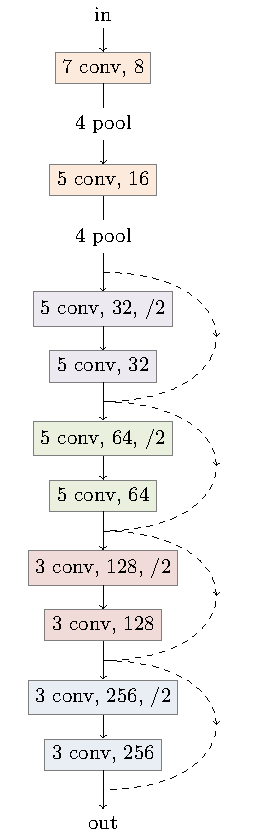
\includegraphics[width=113.6199pt]{machine_learning/images/resnet/custom}
		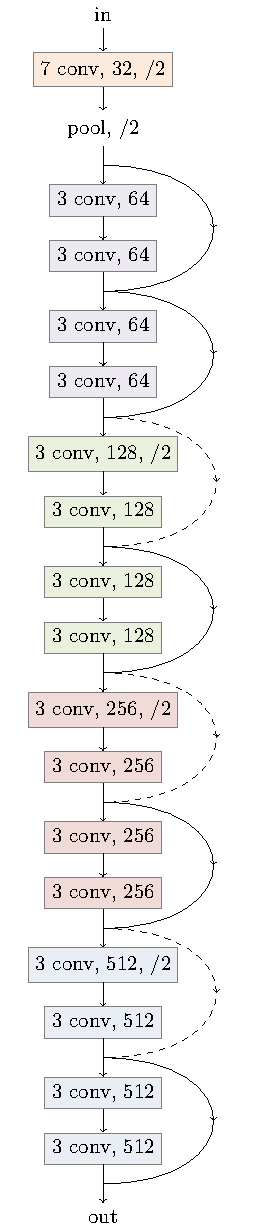
\includegraphics[width=116.11992pt]{machine_learning/images/resnet/resnet18}
		% 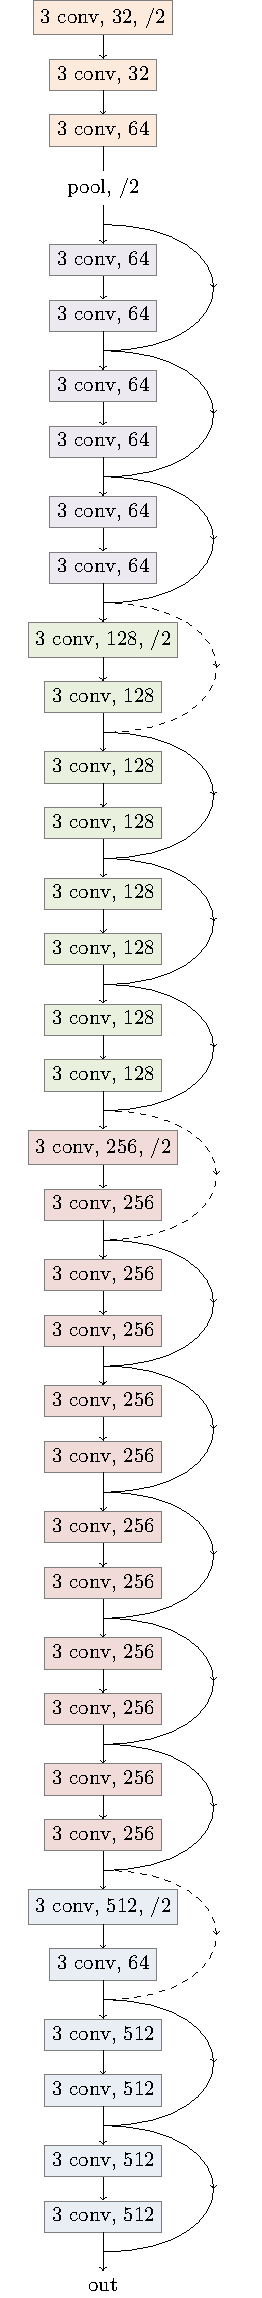
\includegraphics[width=116.11992pt]{machine_learning/images/resnet/resnet34}
	}
	\caption{The custom ResNet architecture that is employed in this work (\emph{left}) and ResNet18~\cite{he2016residual} (\emph{right}). One convolutional block is denoted \enquote{kernel size} conv, \enquote{out channels}, /\enquote{stride}. Skip connections are drawn as arrows. These are dashed if the dimensions do not match.}
	\label{fig:binary:resnet}
\end{figure}

The employed CNN is modeled after ResNet18, the smallest ResNet model with $18$ layers, which is adapted to fit this task's needs (see Fig.~\ref{fig:binary:resnet}). 
\begin{itemize}
\item The number of layers is reduced from $18$ to $12$, decreasing the total model size. The final network has \SI{700}{\kilo\nothing} trainable parameters. 
\item  More aggressive downsampling is implemented to handle the desired long inputs. The model downsamples its input by a factor $256$. For an input of size $3\times\SI{131}{\kilo\nothing}$ (the three detectors are treated as input channels), the model produces an output of shape $256\times512$.
\item  Kernel sizes are increased to enlarge the model's receptive field. This gives a total receptive field of $1766$ or roughly \SI{1}{\second}, which is more than enough to resolve the data's lowest frequencies of \SI{4}{\hertz}.
\end{itemize}
Following the ResNet architecture, \emph{global average pool} is applied over the time dimension of the $256$ feature maps. The output is fed to the classification head, a dense network, 
%\begin{equation}
%	z = \text{Linear}_{1024\rightarrow1}(\text{ReLU}(\text{Linear}_{256\rightarrow1024}(\text{Dropout}(x)))),
%\end{equation}
\begin{align}
	h &= \mathrm{Dropout}(\mathrm{ReLU}(\mathrm{Linear}_{256\rightarrow1024}(x))),\\
	z &= \mathrm{Dropout}(\mathrm{Linear}_{1024\rightarrow1}(h)),
\end{align}
producing single \emph{logit} as output. The dropout probability is \SI{10}{\percent}. A class score obtained through a sigmoid activation,
\begin{equation}
	\hat{y} = \text{Sigmoid}(z) = \frac{1}{1+\e^{-z}},
\end{equation}
which is bounded between $0$ and $1$. 
Note that the model's number of parameters is independent of the input size. This is obviously the case for the kernel parameters, but also for the classification head, since the time information is lost after global average pooling.

% CNN + Transformer hybrid (CNN stays the same)
% explain tokenization
% each downsampled timestep serves as one token
% projected onto model dimension with Conv1d

% Classification token (ViT)
% learned positional encodings

% number of heads and layers
% vram increases quadratically with input size
% 1.7m parameters, no increase with input size

\begin{figure}
	\centering
	\makebox[\textwidth]{
		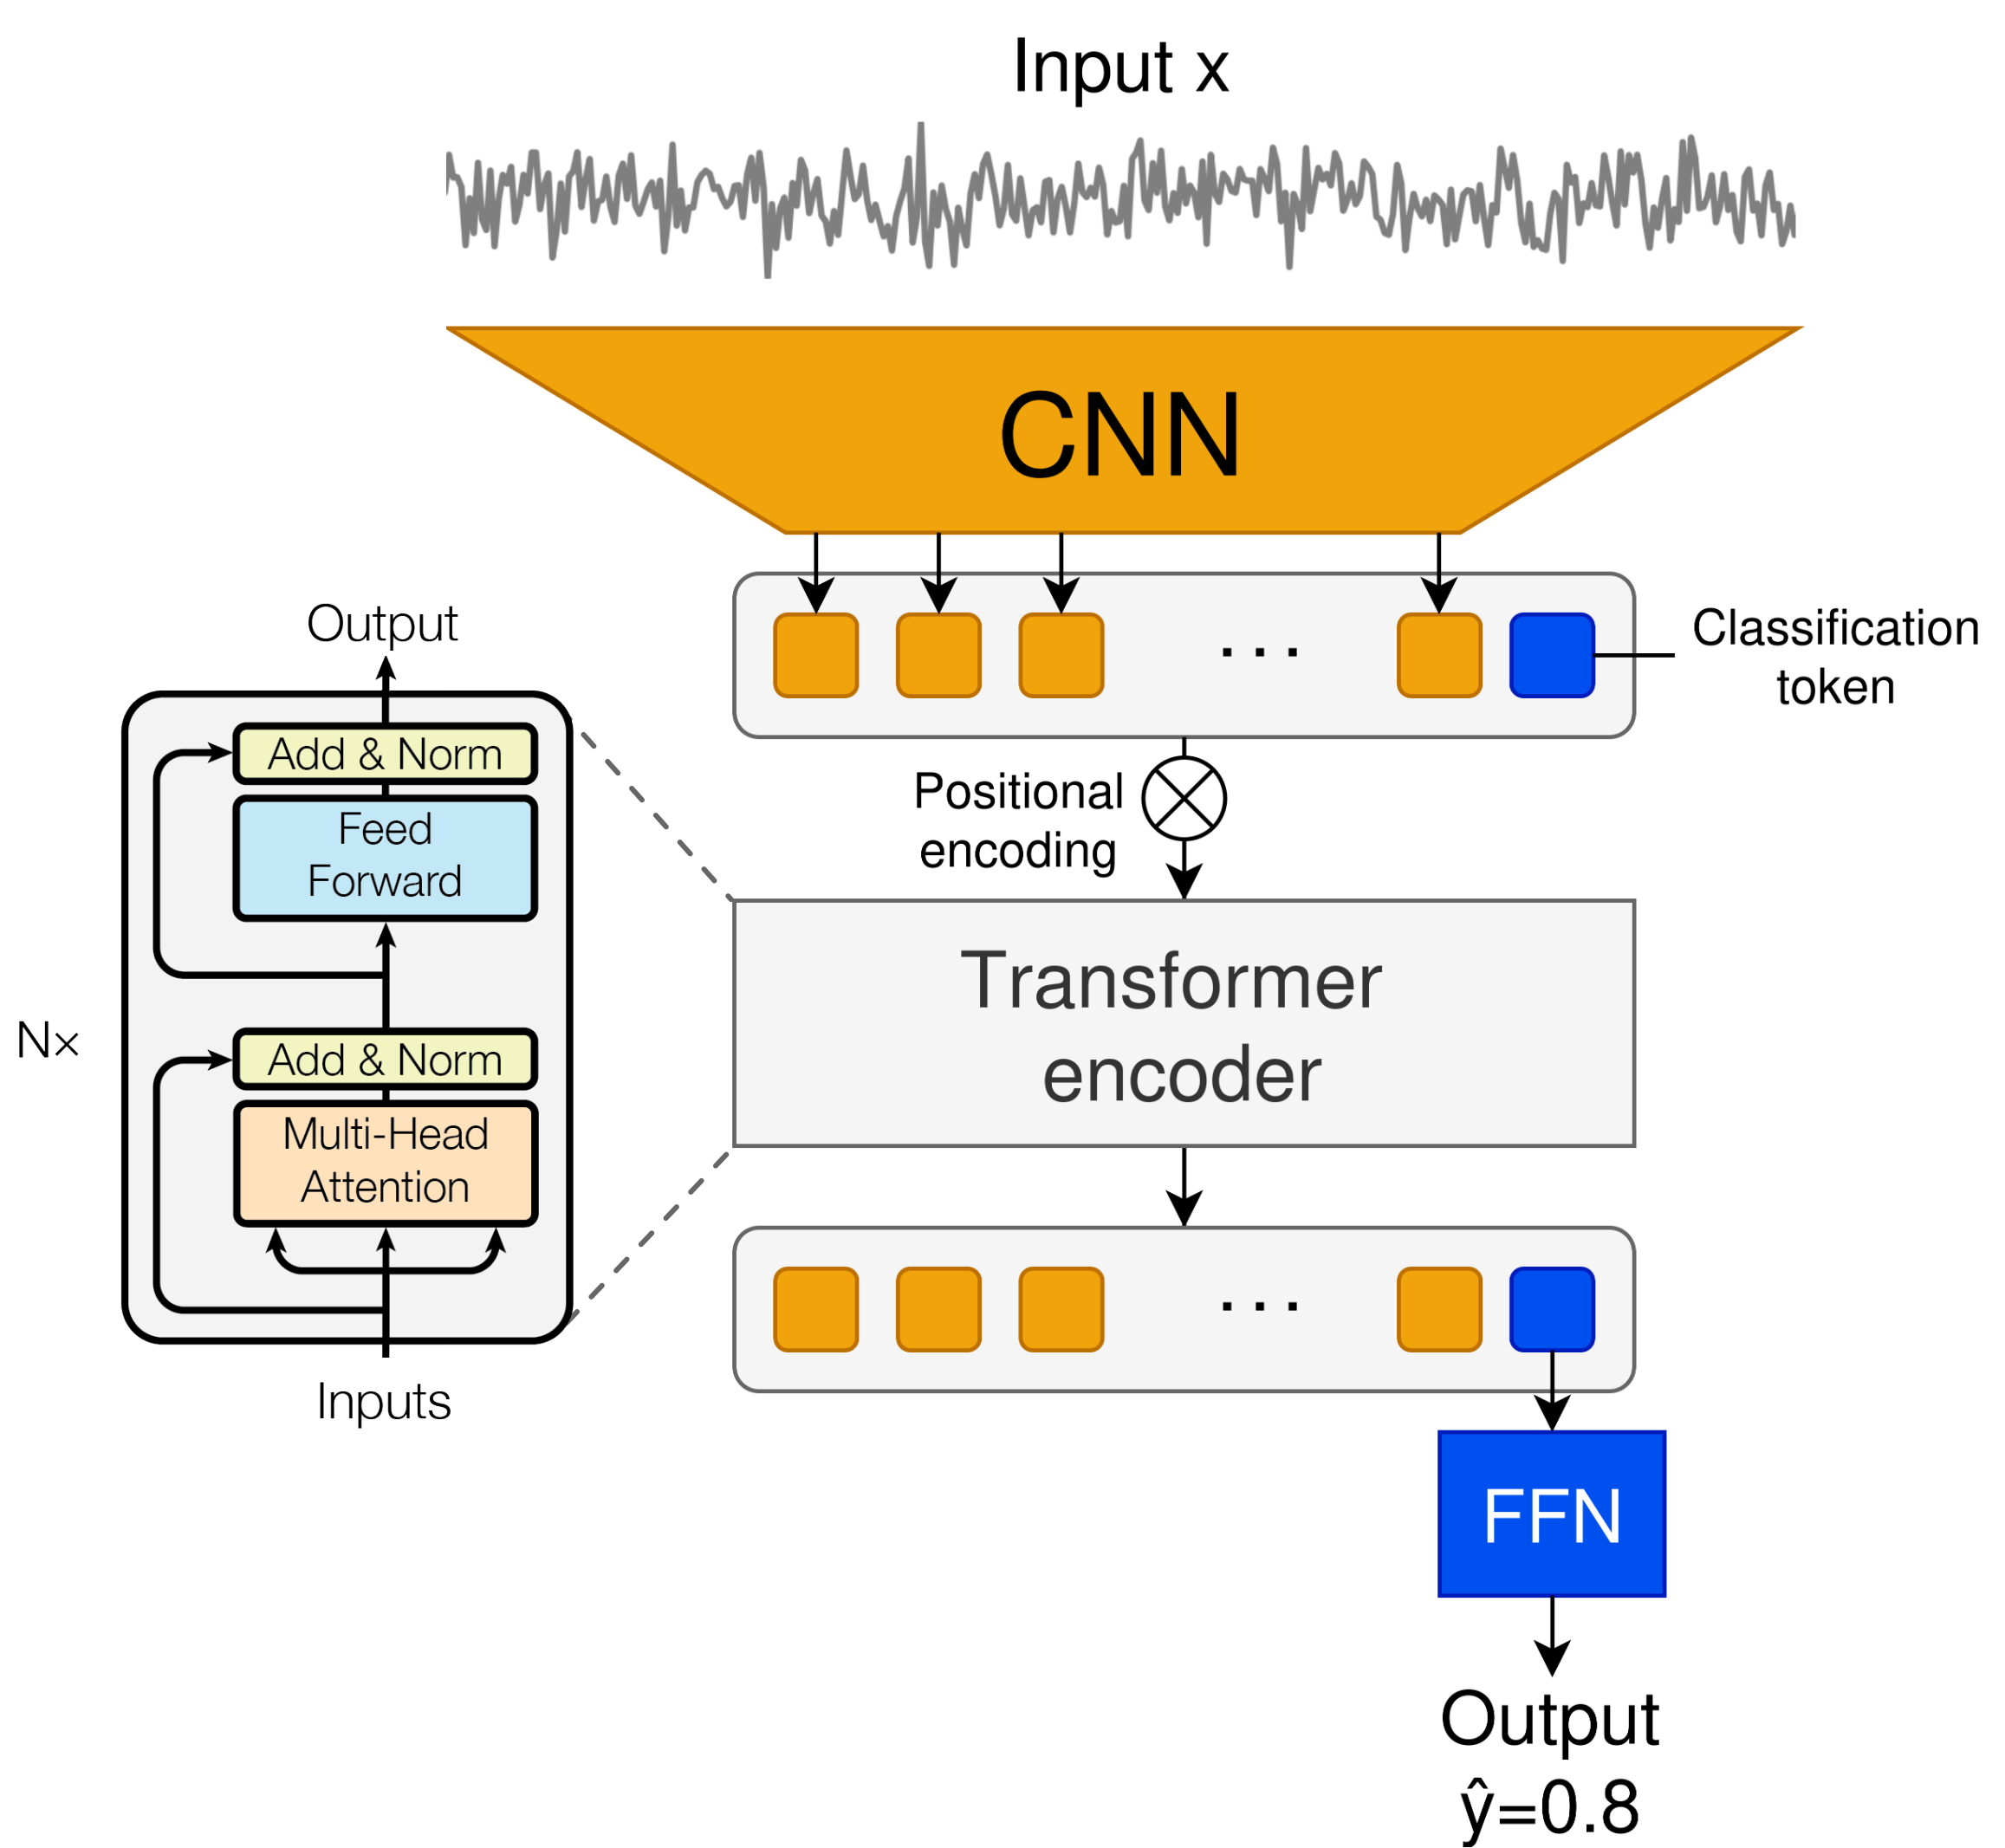
\includegraphics[width=11cm]{binary_classification/images/vit}
	}
	\caption{ViT architecture with an extra classification token.}
	\label{fig:binary:cnn_plus_vit}
\end{figure}

The transformer model, on the other hand, is implemented similarly to the \emph{Vision Transformer} (ViT) \cite{dosovitskiy2021an}, which was originally developed for image classification. The model makes use of the transformer encoder only, which takes as input a number of tokens which are somehow obtained from the input data. The ViT architecture appends an extra learnable \emph{classification token}. This token can attend to the input sequence through the transformer's attention mechanism and its output is read out via a classification head to yield a single class score. See a schematic of the architecture in Fig.~\ref{fig:binary:cnn_plus_vit}.

In NLP, sentences can be straightforwardly tokenized into single words. For other sequential data, appropriate tokenization is less obvious, and there are multiple ways to achieve it. The original ViT model tokenizes 2D images, by splitting them into patches and projecting these onto the desired embedding dimension. For GW data, initial tests showed that this tokenization scheme is too primitive, and results in bad performance. Instead, this work opts for a hybrid approach, where a full CNN serves as the tokenizer. This is outlined in \cite{dosovitskiy2021an} as well, and a similar approach is implemented for transformer based parameter estimation of overlapping signals \cite{Papalini_2025}.
For this CNN tokenizer, the same ResNet model which is described above is employed without average pooling and the classification head. 
For the largest considered input size, this yields $512$ tokens with $256$ channels. 
The resulting tokens represent the input time series in a time-ordered manner, downsampled by a factor of $256$. Each token carries the information of $\approx\SI{1}{\second}$ of data, corresponding to the CNN receptive field size.
A convolution operation with kernel size one reduces the number of channels to the desired embedding dimension $d_\text{embed}=64$.

The classification token is a vector of the same dimension, consisting of learnable parameters. These are initialized randomly. Following \cite{dosovitskiy2021an}, instead of fixed sinusoidal positional encodings, learned position embeddings are added to the input tokens. These are initialized randomly.
The transformer encoder comprises four layers, the attention blocks have eight heads each, and the dense networks' hidden dimension is of size $1024$. The final classification head reads, 
%\begin{equation}
%	z = \text{Dropout}(\text{Linear}_{1024\rightarrow1}(\text{ReLU}(\text{Dropout}(\text{Linear}_{64\rightarrow1024}(\text{LayerNorm}(x)))))),
%\end{equation}
\begin{equation}
\begin{aligned}
	n &= \mathrm{LayerNorm}(x),\\
	h &= \mathrm{Dropout}(\mathrm{ReLU}(\mathrm{Linear}_{64\rightarrow1024}(n))),\\
	z &= \mathrm{Dropout}(\mathrm{Linear}_{1024\rightarrow1}(h)),
\end{aligned}
\end{equation}
which is passed through a sigmoid activation later.
The model employs a dropout probability of \SI{10}{\percent}. (It should be noted that adding a final dropout layer to the classification head is uncommon and unintentional. The results will show that this does not hinder performance, although it leads to unusual learning curves.) The total model size is \SI{1.7}{\mega\nothing} learnable parameters. Apart from the learned embeddings, this is again independent of the input size.

\section{Training}

% minimize bce loss 
% mention logits for numerical stability

As is standard for binary classification tasks, the models are optimized by minimization of the \emph{binary cross entropy} (BCE) loss. Denoting the model output $\hat{y}$ and the target label $y$, this reads,
%\begin{equation}
%	\pazocal{L}_\text{BCE}(y,\hat{y}) = -(y\log{\hat{y}} + (1-y)\log{(1-\hat{y})}).
%\end{equation}
\begin{equation}
	\pazocal{L}_\text{BCE}(y,\hat{y}) = \begin{cases}
		-\log{(1-\hat{y})} & \text{if $y=0$,} \\
		-\log{\hat{y}} & \text{if $y=1$.} 
	\end{cases}
\end{equation}
In practice, the BCE loss is computed directly from the model \emph{logits} $z$ instead, \emph{i.e.}, the unbounded pre-sigmoid outputs, with $\hat{y} = \text{Sigmoid}(z)$. This ensures numerical stability. 

% dataset description 1m train validation with 0.9, 0.1 split and 131k test samples
% even dataset, i.e. 50% positive and 50% negative samples

% optimizer learning rate of 10^-4 batchsize 64
% maximum 100 epochs
% choose weight decay such that models do not overfit drastically

Training datasets are split into \SI{90}{\percent} train and \SI{10}{\percent} validation subsets. Models are trained for a maximum of 100 epochs with the \emph{AdamW} optimizer \cite{loshchilov2019decoupledweightdecayregularization} with a learning rate of \SI{E-4}{}.
The optimizer employs a relatively high weight decay of \SI{0.1}{} to hinder overfitting.
The batch size is $64$, thus each epoch comprises \SI{15}{\kilo\nothing} steps.

% lr scheduler
% CNN: reduce on plateau (similar to magic bullet paper)
% cosine annealing with warmup, standard for transformer architectures

This work utilizes different learning-rate schedules for the two model architectures.
When training the CNN, the learning rate is reduced by a factor of \SI{10}{} if the validation loss has not decreased by at least \SI{0.01}{} in the last 15 epochs. This is similar to \cite{PhysRevD.100.063015}. The ViT is trained with a cosine-annealing learning-rate schedule~\cite{loshchilov2016sgdr}. This is commonly used for transformer architectures. In this case, the learning rate is adjusted by a factor $\alpha$, which depends on the current training epoch and step $x$,
\begin{equation}
	\alpha(x) = \begin{cases}
		\frac{x}{x_0} & x\in[0,x_0), \\
		\frac{1}{2}(1+\cos{\pi\frac{x-x_0}{x_\text{max}-x_0}}) & x\in[x_0,x_\text{max}), \\
		0 & \text{else}.
	\end{cases}
\end{equation}
The schedule yields a linear increase up to $\alpha=1$ at $x_0$, after which $\alpha$ slowly tapers off to zero at $x_\text{max}$. The values $x_0$ and $x_\text{max}$ are set to 2000 steps and 100 epochs respectively.

\begin{figure}
	\centering
	\makebox[\textwidth]{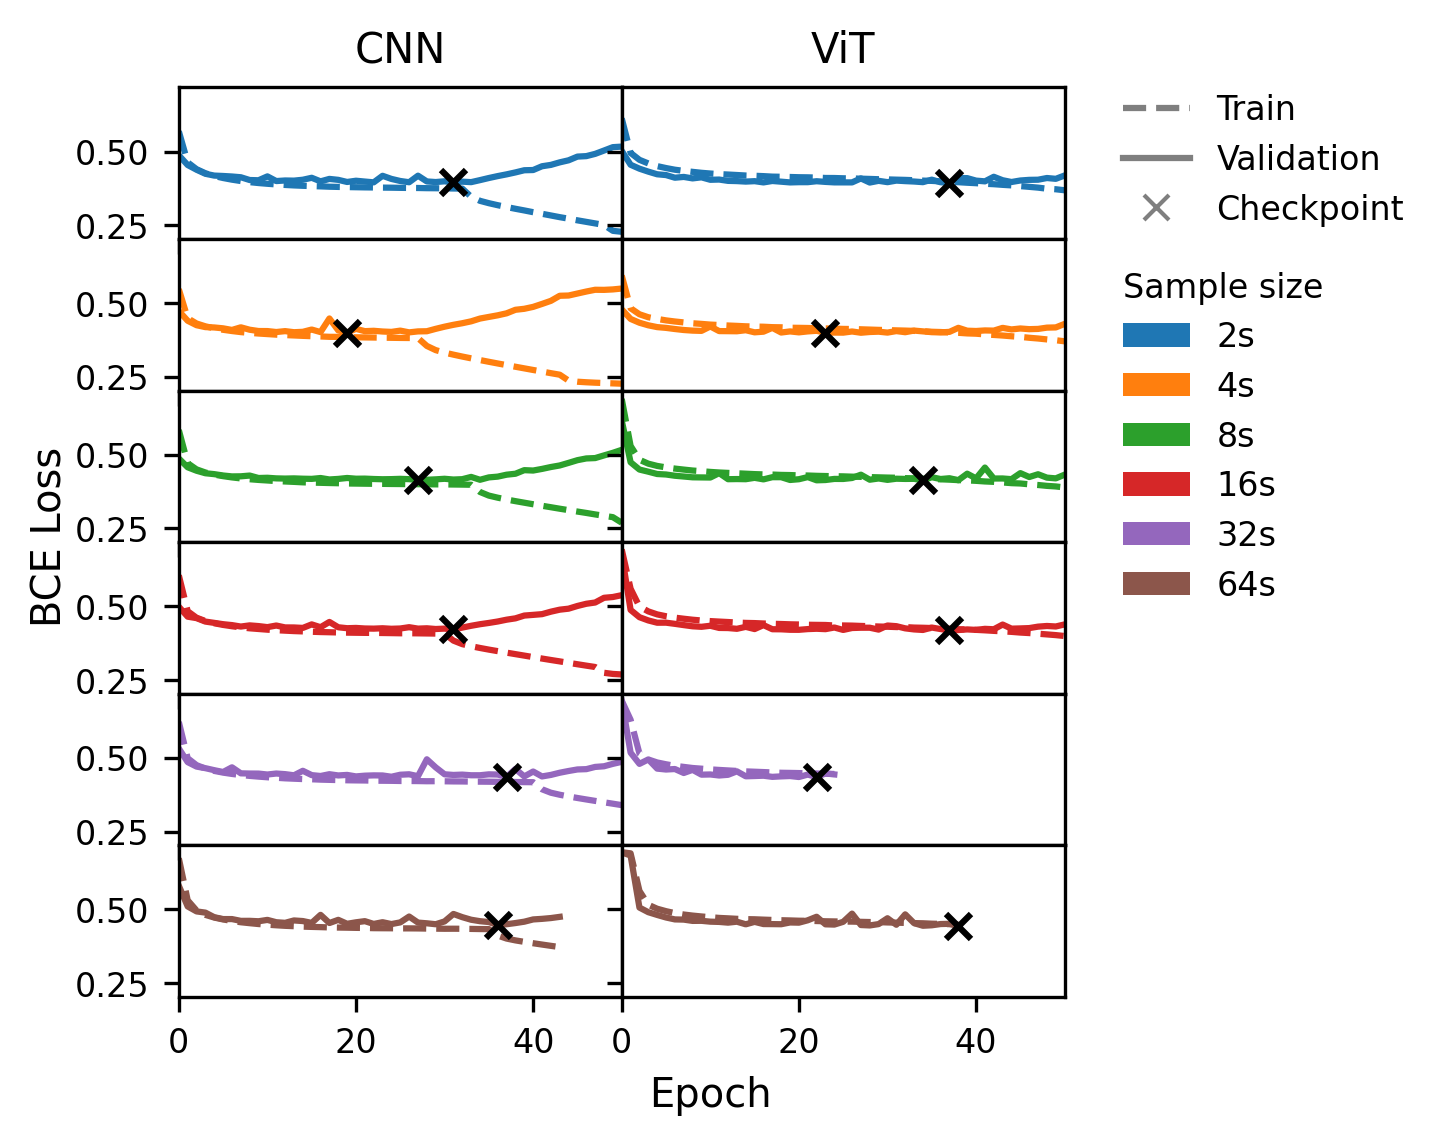
\includegraphics[width=12cm]{binary_classification/plots/learning_curves/curves}}
	\caption{Learning curves. Evolution of the BCE train (\emph{line}) and validation loss (\emph{dashed}) with training epoch for the CNN (\emph{left column}) and ViT models (\emph{right column}). Each row corresponds to one dataset with a different sample size. A marker denotes the minimum validation loss, the point after which overfitting occurs.}
	\label{fig:binary:learning_curves}
\end{figure}

% see learning curves
% all models start to overfit between 20 and 40 epochs
% both cnn and vit have enough parameters for this task
% difference in performance can be interpreted as being caused by model architecture

See the learning curves of all models and datasets plotted in Fig.~\ref{fig:binary:learning_curves}. It can be seen that both the CNN and ViT models start to overfit between 20 and 40 epochs. From this, it can be concluded that both models have enough parameters for this task. Apart from the different learning schedules, differences in performance can be attributed to model architecture only. (Note that, surprisingly, for ViT, the validation loss is in fact smaller than the training loss in the early epochs. This is caused by the unintended final dropout layer, which randomly zeroes the model output with a probability of \SI{10}{\percent}. Since dropout is only applied during training and disabled for evaluation, the model performs better on the validation dataset.)

\section{Performance Comparison}

\begin{figure}
	\centering
	\begin{minipage}[t]{7.5cm}
		\centering
		\makebox[\textwidth]{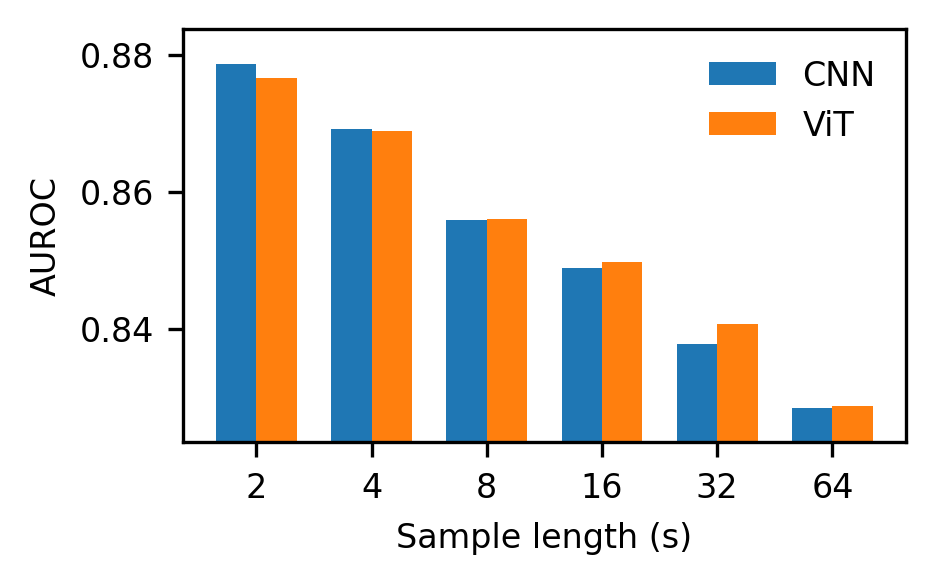
\includegraphics[width=8cm]{binary_classification/plots/comparison/performance}}
		\captionof{figure}{Test dataset AUROC for both models with respect to sample length. Computed over \SI{131}{\kilo\nothing} samples each.}
		\label{fig:binary:comparison}
	\end{minipage}
	\hfill
	\begin{minipage}[t]{7.5cm}
		\centering
		\makebox[\textwidth]{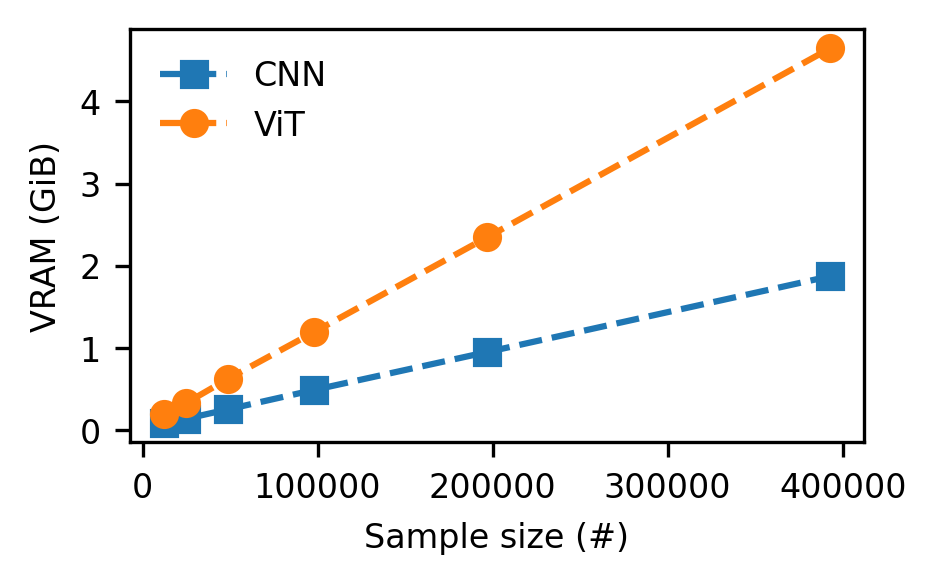
\includegraphics[width=8cm]{binary_classification/images/comparison/vram_size}}
		\captionof{figure}{Peak training VRAM usage with input size. Measured for 64 sample batches on an RTX 4090.}
		\label{fig:binary:vram}
	\end{minipage}
\end{figure}

% checkpointing: choose model parameters with lowest validation loss
% compute roc scores (see fig)
% model performance degrades with larger inputs (expected?)
% CNN and ViT perform equally well 

The performance of both models with respect to dataset sample length is compared. Each model's parameters are chosen from the checkpoint with the lowest validation loss (see Fig.~\ref{fig:binary:learning_curves}). The AUROC is computed over the \SI{131}{\kilo\nothing} sample test datasets, and plotted in Fig.~\ref{fig:binary:comparison}. 

Both models reach $\approx\SI{88}{\percent}$ AUROC for the shortest input size of \SI{2}{\second}. Performance decreases to $\approx\SI{83}{\percent}$ AUROC for \SI{64}{\second}. This decrease was expected and may be attributed to all training datasets having the same size of \SI{1}{\mega\nothing} samples regardless of sample length. The increased size adds complexity, necessitating more training samples.

It can be seen that both the CNN and ViT perform equally well. Contrary to the hypothesis that the attention mechanism handles large inputs more efficiently, this concludes that transformers introduce no performance gain in this context. 
% Still, the transformer architecture achieves comparable performance. 
Although its memory usage is higher compared to the CNN, with at most 512 tokens for \SI{64}{\second} samples, it is far from the quadratic regime expected from the attention mechanism (see Fig.~\ref{fig:binary:vram}). This is an important intermediate result before dealing with overlapping signals.

\section{Parameter Biases}

% look at performance on 64s samples for one model (vit) more closely
% check for biases (from dataset)
% diagnostic check

Having established that both models can process the desired input size, the performance of the ViT model on \SI{64}{\second} samples is studied in more detail.  The goal is to perform diagnostic checks before moving to overlapping waveforms. In particular, these are checks for any biases the model might have learned with respect to the injected waveform's parameters. Since both models perform similarly, the assumption is made that biases mostly depend on the data itself and not the model type. The ViT model is chosen for this analysis because its attention weights provide an additional diagnostic of which parts of the input contribute to the classification.

% choose arbitrary threshold 
% see roc curve
% minimize distance to (FPR=0, TPR=1)

\begin{figure}
	\centering
	\makebox[\textwidth]{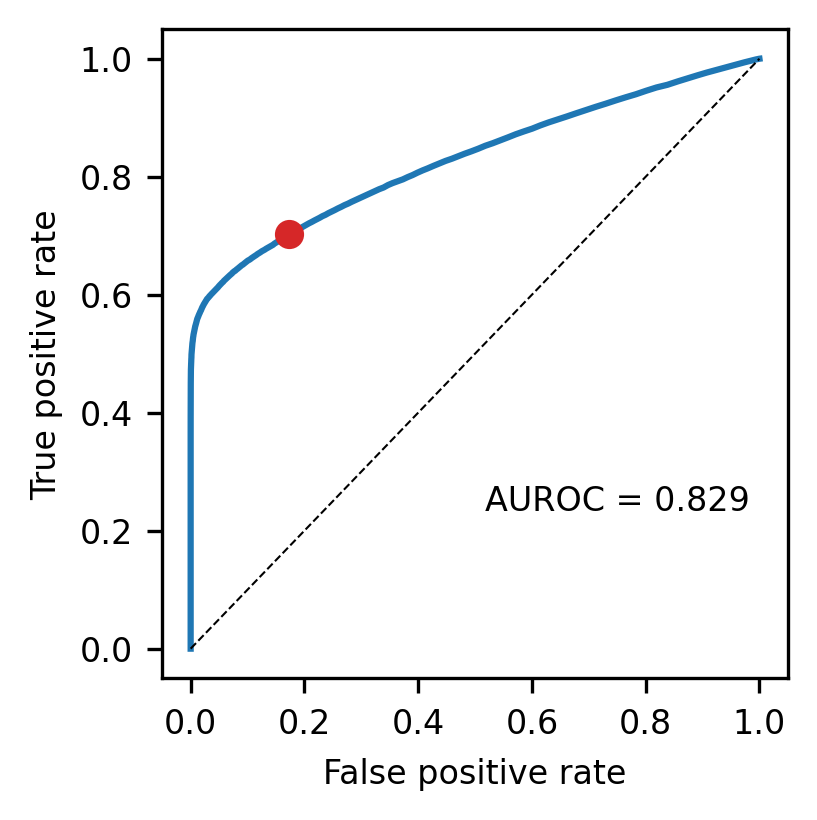
\includegraphics[width=7cm]{binary_classification/plots/auroc}}
	\caption{ViT ROC for \SI{64}{\second} samples. The dotted line shows the performance of a random classifier, which has \SI{50}{\percent} AUROC. The red dot shows the chosen operating point.}
	\label{fig:binary:auroc}
\end{figure}

Employing this model as a binary classifier requires choosing an appropriate \emph{operating point} first. This means setting the threshold to yield some FPR and TPR. To this end, the ROC is consulted in Fig.~\ref{fig:binary:auroc}, which shows all the possible operating points. Note that there are many points with a FPR close to zero while reaching TPR up to $\approx\SI{50}{\percent}$. This reveals that a large fraction of target positive samples are easy to identify for the network. This is promising for GW searches, which focus on minimizing the false alarm rate while reporting as many signals as possible.

Again, as this study does not aim to implement a proper search, and is interested in diagnostic checks for now, the operating point can be chosen more or less arbitrarily. One such way is to find the threshold such that the resulting operating point has minimum distance to a perfect classifier with zero FPR and unit TPR. Then, the desired or optimal threshold is,
\begin{equation}
	z_\text{opt} = \argmin_{z} \sqrt{\text{FPR}(z)^2 + (1-\text{TPR}(z))^2},
\end{equation}
resulting in a threshold of \SI{27.5}{\percent}. Model predictions below \SI{27.5}{\percent} are labeled negative and positive else. This gives \SI{17.4}{\percent} FPR and \SI{70.2}{\percent} TPR. \SI{17.4}{\percent} of all noise samples are incorrectly predicted to contain a signal, and \SI{70.2}{\percent} of all injection samples are correctly identified. 
% See the confusion matrix in Fig.~\ref{fig:}.

% explain detection ratio 

The metric by which the model's performance with respect to the waveform parameters is evaluated is the \emph{detection ratio}. That is, how many signals (which have these waveform parameters) are found? In this case, this is simply the TPR. 

\begin{figure}
\centering
\begin{subfigure}{0.48\textwidth}
	\centering
	\makebox[\textwidth]{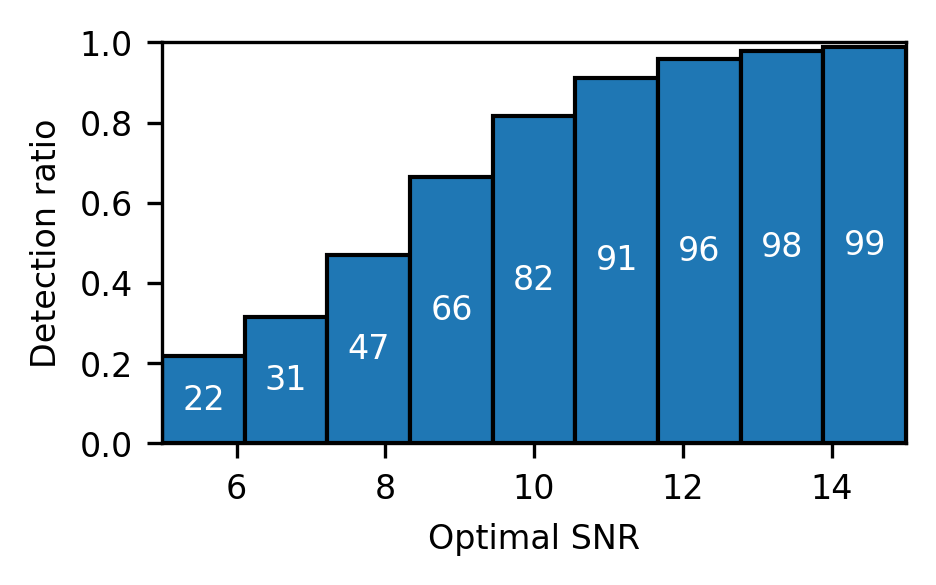
\includegraphics[width=8cm]{binary_classification/plots/snr}}
	\caption{}
	\label{fig:binary:snr}
\end{subfigure}
\hfill
\begin{subfigure}{0.48\textwidth}
	\centering
	\makebox[\textwidth]{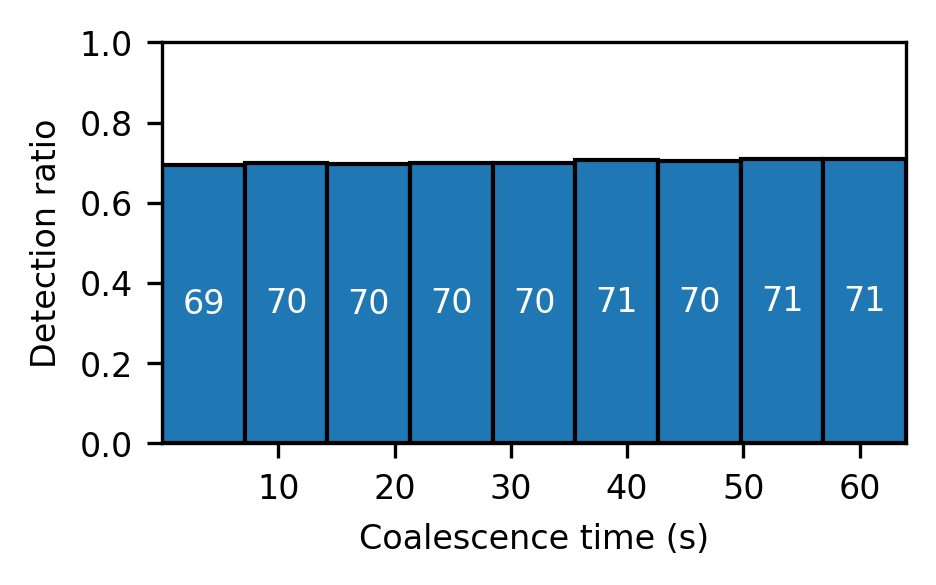
\includegraphics[width=8cm]{binary_classification/plots/merger_time}}
	\caption{}
	\label{fig:binary:merger_time}
\end{subfigure}
\begin{subfigure}{0.48\textwidth}
	\centering
	\makebox[\textwidth]{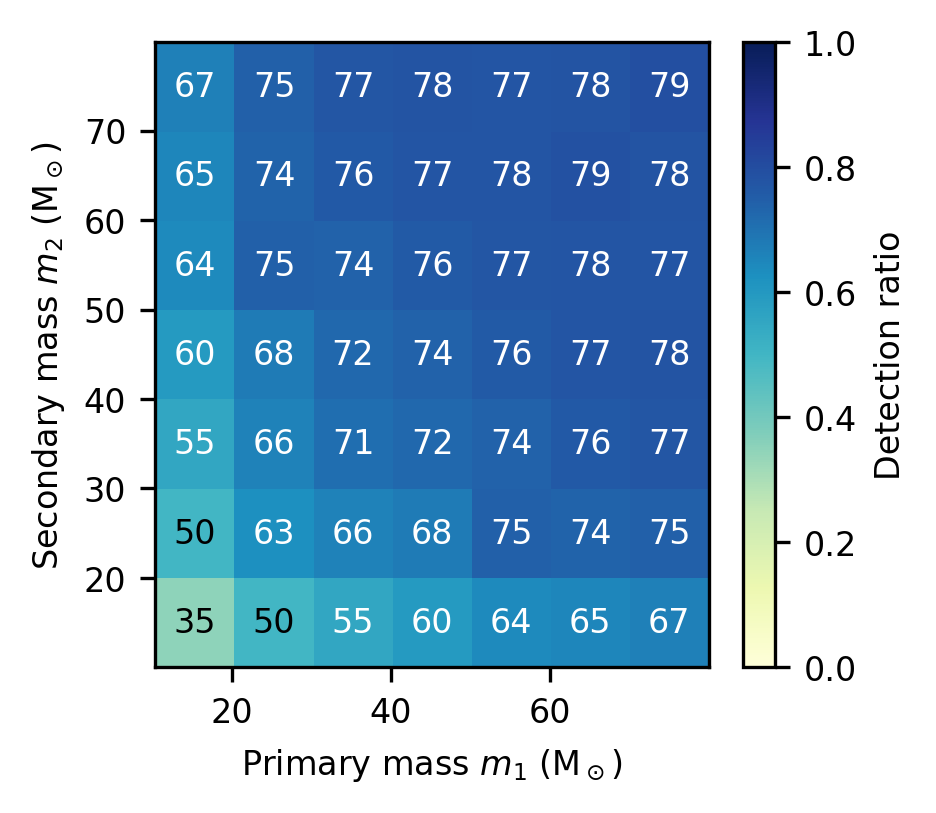
\includegraphics[width=8cm]{binary_classification/plots/mass}}
	\caption{}
	\label{fig:binary:mass}
\end{subfigure}
\hfill
\begin{subfigure}{0.48\textwidth}
	\centering
	\makebox[\textwidth]{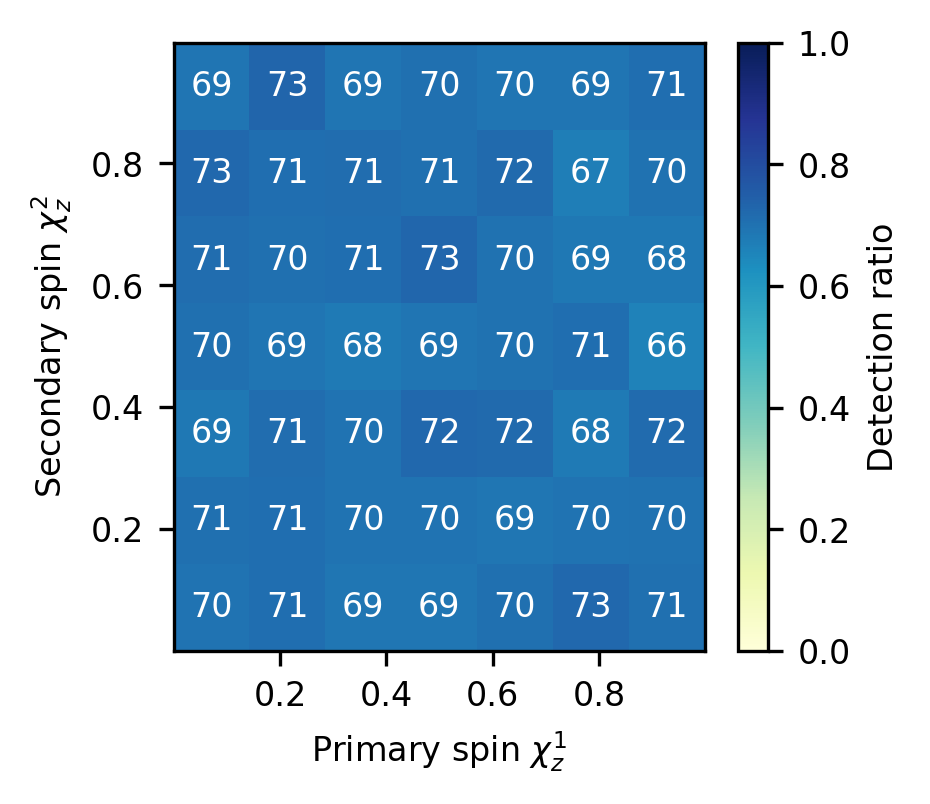
\includegraphics[width=8cm]{binary_classification/plots/spins}}
	\caption{}
	\label{fig:binary:spin}
\end{subfigure}
\caption{Detection ratio as a function of various signal parameters: SNR (\emph{a}), coalescence time (\emph{b}), the two objects masses (\emph{c}) and spins (\emph{d}). Computed over a total of \SI{66}{\kilo\nothing} test samples. In (\emph{c}), the values are mirrored along the diagonal for visualization purposes. Labels are rounded to the nearest integer or the first decimal place. Uncertainties are not plotted.}
\end{figure}

% snr plot
% detection ratio increases with snr
% expected
% good because it verifies that the models really learn to identify GW signals instead of picking up on some giveaways caused by faulty data

It is natural to first consider the model's performance with respect to SNR. Test samples are subdivided into nine SNR bins in $[5, 15]$, and the detection ratio is computed separately for each bin. The result is shown in Fig.~\ref{fig:binary:snr}. In this case, half of the test dataset is considered consisting of only positive samples containing a signal. Thus, each bin consists approximately $N=\SI{7}{\kilo\nothing}$ test samples. Assuming a binomial distribution with probability $p$, \emph{i.e.}, the detection ratio, then each bin has a standard deviation of $\sigma = \sqrt{p(1-p)/N}$.

It can be seen that the model achieves close to perfect detection ratios of \SI{99.0(1)}{\percent} for the loudest signals, indicating that these signals are easily identified. For the faintest signals, the detection ratio decreases to \SI{21.7(5)}{\percent}. This trend is expected: low-SNR signals are harder to distinguish from noise. It is also a useful sanity check, since it suggests that the network output is correlated with the signal loudness rather than with any artefacts in the simulated data.

% merger time plot
% detection ratios only varies slightly with merger time
% no biases with merger time 
% slight decrease for mergers closer to 0, because less of their signal lies in the sample (check significance)
% 9 bins, 131k/9 samples per bin, sigma = sqrt(0.7(1-0.7)/(131k/9)) = 0.4%

The same analysis is applied to the signal coalescence time, i.e. the position of the merger within the sample. See the results in Fig.~\ref{fig:binary:merger_time}. The network achieves detection ratios $\approx\SI{70}{\percent}$ regardless of coalescence times. A small decrease is noticeable from $\SI{71.0(5)}{\percent}$ for signals whose merger lies close to the \emph{right} sample edge down to $\SI{69.4(5)}{\percent}$ closer to the \emph{left} edge. A decrease is expected, since less of the signal inspiral phase is contained in the sample in this case. Here, the effect is statistically insignificant, suggesting that predictions are made mostly based on the signals' late inspiral and merger phase, rather than by the full waveform.

% mass plot
% detection ratio decreases with lower mass
% more snr lies in the inspiral for low mass inspirals (see plot)
% maybe network only focuses on merger? check attention weights

Because the shape of CBC waveforms depends largely on the component masses $m_1, m_2$ (compare Eq.~\ref{eq:gravitational_waves:cbc_waveform}), it makes sense to investigate model performance as a function of these. To this end, both the primary and secondary masses are subdivided into seven bins in $[\SI{10}{\solarmass}, \SI{80}{\solarmass}]$. From this, a $7\times7$ matrix is constructed with rows corresponding to the primary mass $m_1$ bins and columns to the secondary mass $m_2$ bins. The detection ratio is computed separately for each entry. Since $m_1>m_2$, the upper triangular half of that matrix contains no samples. To yield a full matrix, entries are mirrored along the diagonal. The result is plotted in Fig.~\ref{fig:binary:mass}.

The plot exhibits two notable features, which are both statistically significant. First, the detection ratio increases with total mass, from $\SI{35(1)}{\percent}$ for the lowest total masses $M = m_1+m_2 \approx\SI{20}{\solarmass}$ up to $\SI{79(1)}{\percent}$ for the highest masses $\approx\SI{160}{\solarmass}$. Second, along diagonals of approximately constant total mass, the detection ratio decreases with \emph{mass ratio} $q = m_1 / m_2$. For example, along the center diagonal with total mass $M \approx \SI{90}{\solarmass}$, the detection ratio decreases from $\SI{74(1)}{\percent}$ for equal masses, \emph{i.e.}, $q\approx1$ to $\SI{66.5(9)}{\percent}$ for mass ratios close to $q\approx8$.

\begin{figure}
	\centering
	\makebox[\textwidth]{
		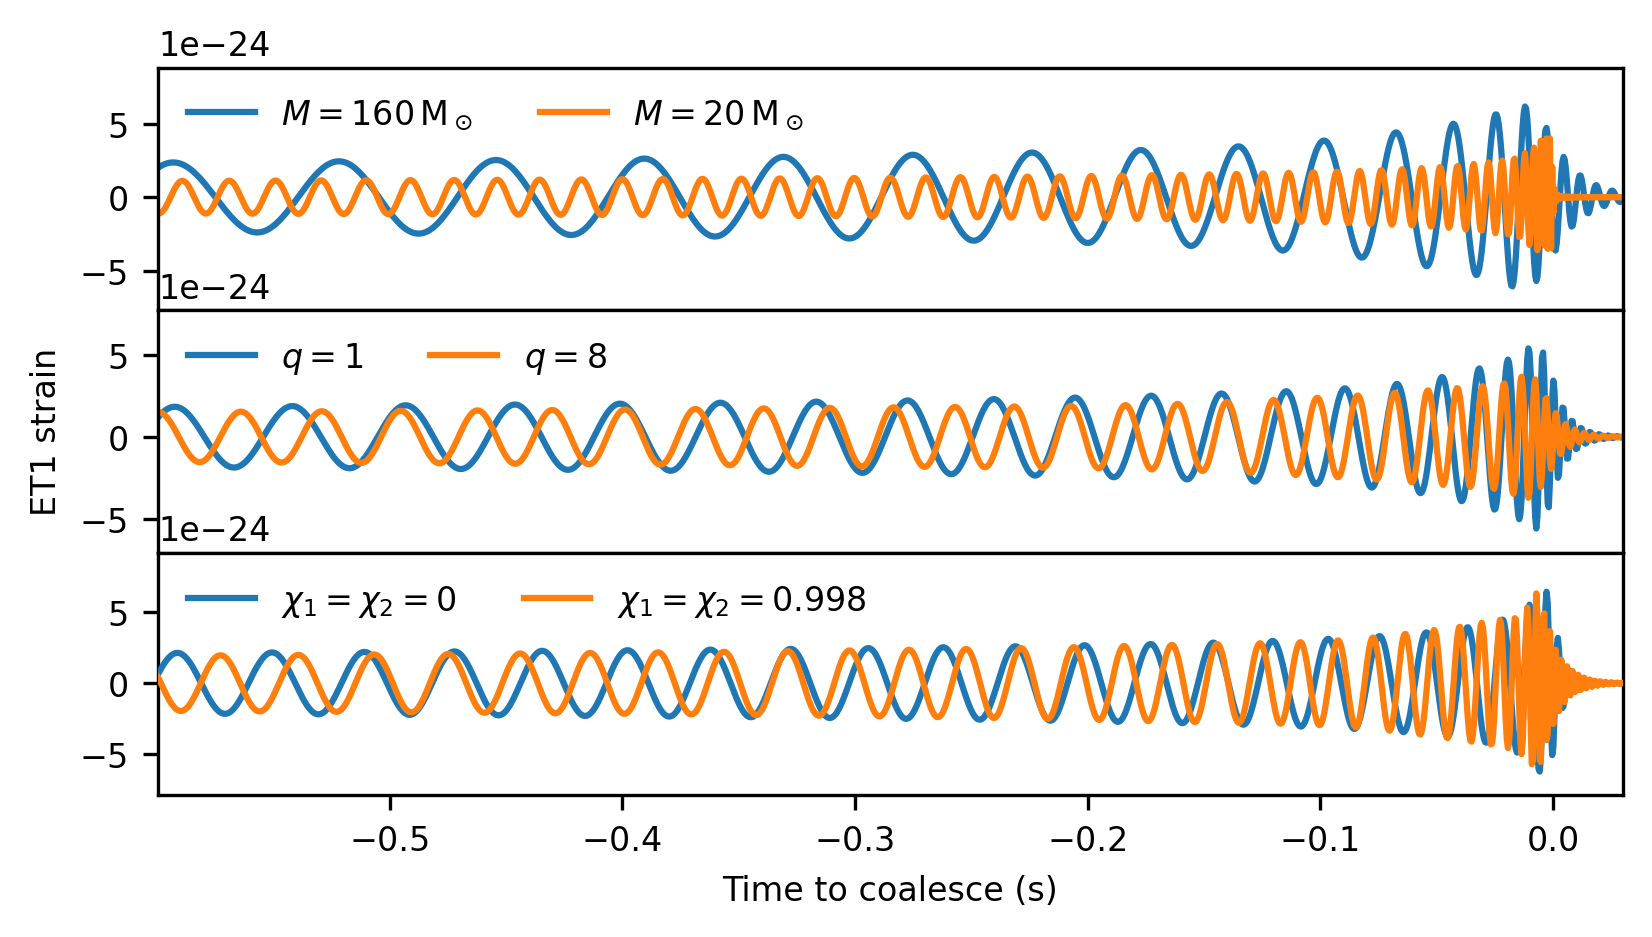
\includegraphics[width=16cm]{binary_classification/images/parameters/waveforms}
	}
	\caption{Equal-SNR ($\rho=10$) signals with different parameters. For visualization purposes, only the ET1 channel is plotted. Each row shows two waveforms with different total mass (\emph{top}), mass ratio (\emph{middle}), and spins (\emph{bottom}) and otherwise equal parameters.}
	\label{fig:binary:low_mass_waveform}
\end{figure}

Both effects can be understood from the dependence of the waveform duration on chirp mass. At leading order, the duration scales as $\tau \propto 1/\pazocal{M}^\frac{5}{3}$ (see Eq.~\ref{eq:matched_filtering:signal_duration}).
The chirp mass can be written as
\begin{equation}
	\pazocal{M} = \frac{(m_1m_2)^\frac{3}{5}}{(m_1+m_2)^\frac{1}{5}} = \frac{q^\frac{3}{5}}{(1+q)^\frac{6}{5}}\,M.
\end{equation}
Therefore, lower total masses and larger mass ratios correspond to smaller chirp masses and hence longer signals. The observed decrease in detection ratio can thus be interpreted as a degradation of model performance for longer-duration signals. 

For these longer waveforms, SNR lies mostly in the long inspiral phase. If two signals have equal SNR, but one is longer, the longer waveform will have a smaller total amplitude. See Fig.~\ref{fig:binary:low_mass_waveform} where equal-SNR waveforms with different masses are compared. 
Assuming sufficient template size, matched filtering detects these signals equally well, regardless of signal amplitude, since their SNR is the same. For neural networks, however, longer and lower-amplitude signals appear to be more challenging.

% spin plot
% 7^2 bins, 131k/7^2 samples per bin, sigma = sqrt(0.7(1-0.7)/(131k/7^2)) = 0.9%
% no biases -> good

Finally, the detection ratio is checked against the remaining intrinsic waveform parameter, each black hole's spin z-component. Remember that only aligned-spin BBHs are considered in this work, which have vanishing spin x and y-components. Similar to the mass analysis, the primary and secondary spins are subdivided into seven bins in $[0,0.998]$, forming a $7\times7$ matrix. Since the spin values are drawn independently, each entry contains \SI{2400}{\nothing} samples. The result is plotted in Fig.~\ref{fig:binary:spin}. A detection ratio of $\approx\SI{70}{\percent}$ is achieved throughout. No clear trend is visible, and values vary between \SI{66.1(1.3)}{\percent} and \SI{72.9(1.2)}{\percent}, which is a difference of $3.8\,\sigma$. Thus it can be concluded that model performance is agnostic to the binary component spins. This is consistent with the earlier result that performance is mostly limited by signal length and amplitude. By simulating equal-SNR waveforms with different spins (see Fig.~\ref{fig:binary:low_mass_waveform}), it can be seen that, contrary to the effect of different component masses, the waveforms vary very little with spin.
 
\section{Attention Analysis}

Up to now, the results suggest that the neural network makes predictions mostly based on the waveform's merger phase where the amplitude is maximum. Because of this, performance is independent of injection time, but degrades for longer waveforms where most of the SNR lies in the inspiral part. As this analysis uses the ViT model, this hypothesis can be validated by checking the model's attention weights.

% new 65k sample test dataset with fixed merger time at 60s to gather some statistics
% mean attention weights of classification token
% bin into snr ranges
% see plot

For this, a new test dataset is simulated with \SI{66}{\kilo\nothing} positive, \emph{i.e.}, signal containing, samples with constant coalescence time. The sample size is \SI{64}{\second} and signals are always injected with a coalescence time of \SI{60}{\second}. The simulation parameters are otherwise unchanged. 

To check what lead the ViT model to make its prediction, the transformer encoder weights are investigated. These correspond to a $513\times513$ self-attention matrix for the $512$ time series tokens and the extra classification token. Each row of this matrix corresponds to one target or output token, and each entry of that row contains the weight that token assigns to the source or input tokens. 

Since the final prediction only depends on the classification token, only the weights that this token assigns to the other $512$ time series tokens are of interest. These weights correspond to the first $512$ entries in the last row of the attention matrix. After CNN tokenization, the resulting tokens still represent the input series in a time ordered, albeit downsampled, fashion. Thus, the considered $512$ classification token attention weights can be related to the input time series to show which part of the waveform is deemed important for the prediction.

\begin{figure}
	\centering
	\makebox[\textwidth]{
		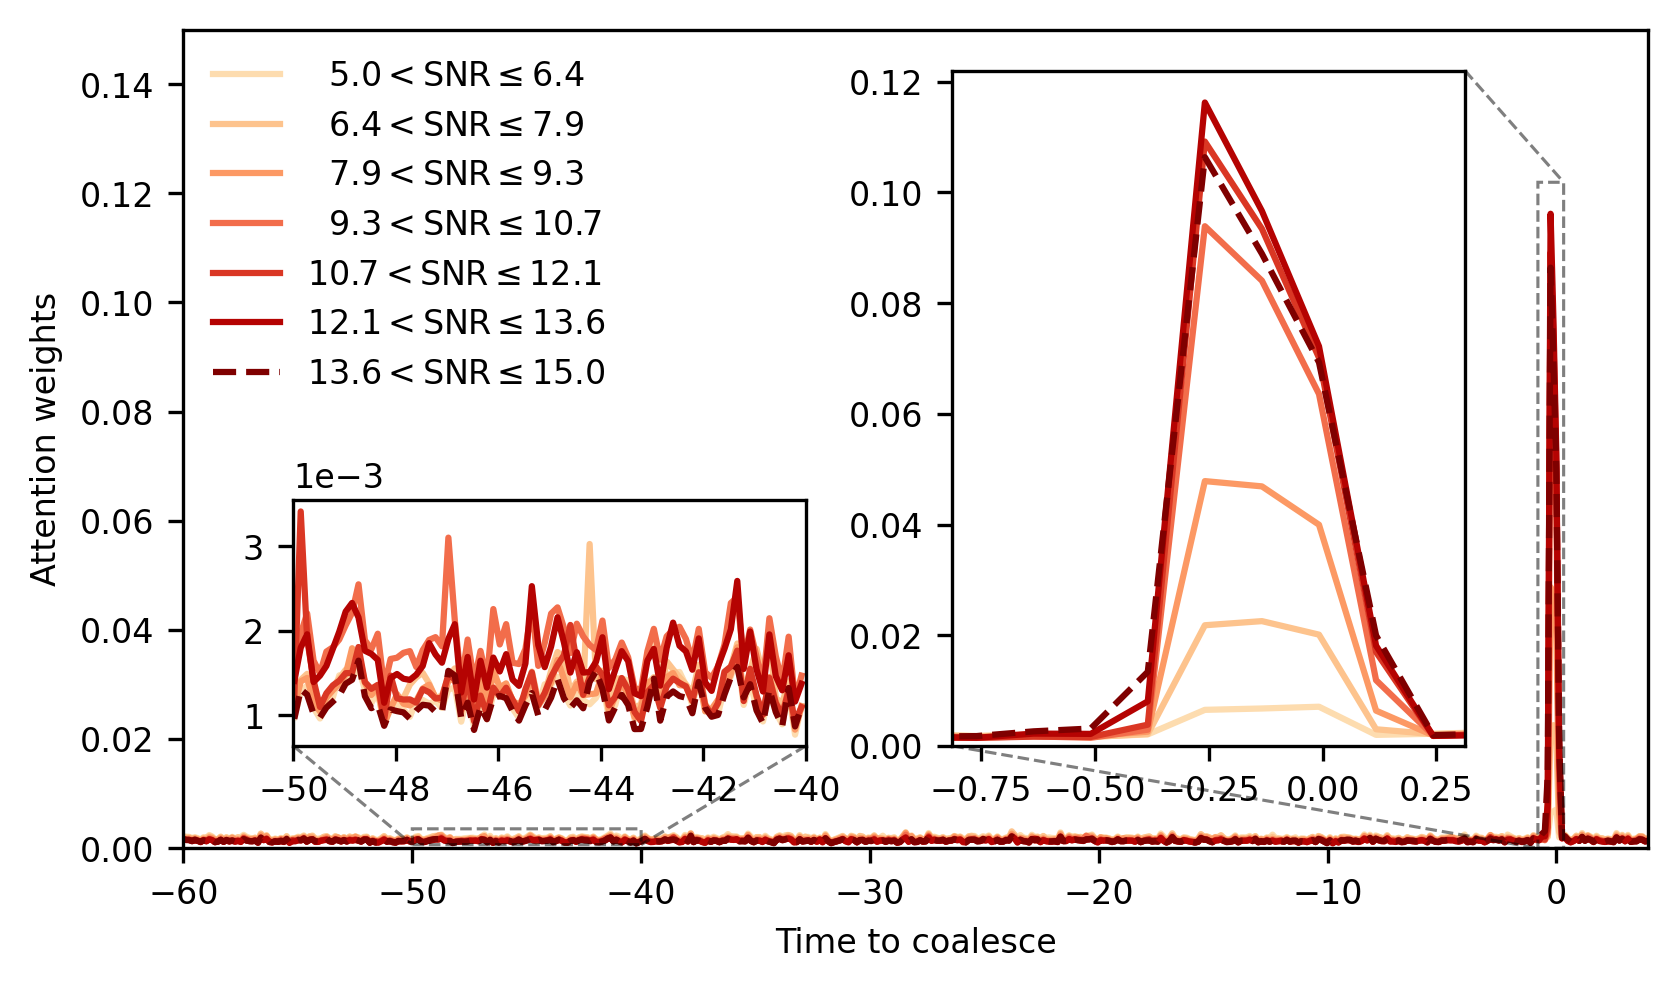
\includegraphics[width=16cm]{binary_classification/plots/attention/attention}
	}
	\caption{Attention weights assigned by the ViT classification token to the input time series tokens. Averaged over multiple samples with fixed merger time. Seven SNR bins are considered. The corresponding weights are plotted in different colors. Darker colors signify louder signals. The highest-SNR weights are dashed for clarity.}
	\label{fig:binary:attention}
\end{figure}

In particular, the last encoder layer's weights are investigated, and these averaged over all eight heads.
To gather some statistics, these weights are again averaged over multiple samples. To this end, the test dataset is divided into seven SNR bins in $[5, 15]$, each containing \SI{9}{\kilo\nothing} samples. For each subset, and for each timestep, the weights are the averaged separately. See the result in Fig.~\ref{fig:binary:attention}.

% on average, attention focuses only on the last 0.5s until merger
% peak increases in height with snr
% except for last bin where the peak gets slightly more broad, i.e. more of the waveform is payed attention to, but this effect is very minor

From this plot, it becomes clear that the attention is very \emph{sparse}. Most attention is paid to the $\approx\SI{1}{\second}$ around the merger, leaning more towards the inspiral instead of the ringdown phase. The height of that peak grows for louder signals, from $\approx\SI{E-2}{}$ for low SNRs up to  $\approx\SI{E-1}{}$ for high SNRs. Outside that region, the weights are smaller on average with values of order $\pazocal{O}(\SI{E-3}{})$. 

% verifies that attention mechanism works 
% again data is propably not faulty
% although large input size, network does not capture the waveform fully
% maybe increase performance by making attention less sparse?
% curriculum learning

This verifies that the model prediction is based mostly on the high amplitude merger phase of the signal. From this, it is clear that networks struggle with long-duration waveforms since their maximum amplitude is lower. Although the network is able to process the whole \SI{64}{\second} sample size, only a fraction of that information is used to make predictions. 

Again, the attention weights serve as a useful sanity check. It can be verified that the transformer is implemented correctly and that the attention mechanism works as expected. Further, the plot suggests that the network does not pick up on any possible artefacts in the data, and that predictions are based on the signal's merger phase.

\section{Summary}

This study shows that both the CNN and ViT models can process the required sample size of \SI{64}{\second}. A performance decrease is observed when going to larger inputs, which is attributed to training data size. No clear performance advantage of the transformer model is observed in this single-signal setting. Further analysis shows that models struggle for long-duration waveforms, such as low mass inspirals and high mass-ratio inspirals. Although the networks manage to process the full \SI{64}{\second} sample, they seem to focus mostly on the high amplitude merger phase, which is less pronounced in long signals.

% models decrease in performance with input size
% both cnn and vit can process long inputs
% no clear performance gain from attention mechanism
% no biases in dataset
% data not faulty
% vit focuses only on last part of merger neglecting the long inspiral
% performance decreases for low mass inspirals